\chapter{Generalized Minimum Residual Method (GMRES)}
Let $\mathcal{K} = \mathcal{K}_m(A, \mathbf{r}_0)$ and $\mathcal{L}_m = A\mathcal{K}_m$.
This chapter describes the GMRES algorithm (Generalized Minimum Residual), an important Krylov-subspace method for solving nonsymmetric linear systems. We present the least-squares formulation, the practical QR/Givens implementation used in practice, a short worked example, and a visualisation of residual decay.
\begin{align*}
    \mathbf{r}_m                     & = \mathbf{b} - A\mathbf{x}_m                                                                                                                                                                    \\
    \|\mathbf{b} - A\mathbf{x}_m\|_2 & = \min_{\mathbf{x} \in \mathbf{x}_0 + \mathcal{K}_m} \|\mathbf{b} - A\mathbf{x}\|_2                                                                                                             \\
    \mathbf{x}                       & \in \mathbf{x}_0 + \mathcal{K}_m \quad \Rightarrow \quad \mathbf{x} = \mathbf{x}_0 + V_m \mathbf{y}_m,\quad \mathbf{y}_m \in \mathbb{R}^m                                                      \\
    \mathbf{r}                       & = \mathbf{b} - A\mathbf{x} = \mathbf{b} - A(\mathbf{x}_0 + V_m \mathbf{y}_m) = \mathbf{r}_0 - AV_m \mathbf{y}_m                                                                                 \\
                                     & = \mathbf{r}_0 - V_{m+1} \overline{H}_m \mathbf{y}_m                                                                                                                                            \\
                                     & = V_{m+1}\big(\beta \mathbf{e}_1 - \overline{H}_m \mathbf{y}_m\big), \qquad \beta = \|\mathbf{r}_0\|_2                                                                                         \\
    \|\mathbf{r}\|_2                 & = \|V_{m+1}(\beta \mathbf{e}_1 - \overline{H}_m \mathbf{y}_m)\|_2 = \|\beta \mathbf{e}_1 - \overline{H}_m \mathbf{y}_m\|_2
    \quad\text{(columns of $V_{m+1}$ orthonormal)}                                                                          \\
    \mathbf{y}_m                     & = \arg\min_{\mathbf{y} \in \mathbb{R}^m} \|\beta \mathbf{e}_1 - \overline{H}_m \mathbf{y}\|_2                                                                                                   \\
    \mathbf{x}_m                     & = \mathbf{x}_0 + V_m \mathbf{y}_m
\end{align*}
We therefore solve the overdetermined system ($m<n$)
\[
    \overline{H}_m \mathbf{y} \approx \beta \mathbf{e}_1
\]
via a least squares solve, efficiently obtained by QR factorization of the upper Hessenberg matrix $\overline{H}_m$ using Givens rotations.

\section{QR factorization approach}
Since $\overline{H}_m\in\mathbb{R}^{(m+1)\times m}$ is upper Hessenberg, we compute a thin QR
\[
    \overline{H}_m = Q_{m+1}\,\widetilde{R}_m,
\]
where $Q_{m+1}\in\mathbb{R}^{(m+1)\times(m+1)}$ is orthogonal and
\[
    \widetilde{R}_m = \begin{bmatrix} R_m \\ \mathbf{0}^\top \end{bmatrix},\qquad
    R_m\in\mathbb{R}^{m\times m}\ \text{upper triangular}.
\]
Set
\[
    \bar{\mathbf{g}}_m = Q_{m+1}^\top\beta\mathbf{e}_1 = [\gamma_1,\gamma_2,\dots,\gamma_{m+1}]^\top.
\]
Then the least squares problem becomes
\begin{align*}
    \beta\mathbf{e}_1 - \overline{H}_m\mathbf{y}
    &=
    Q_{m+1}\big(\bar{\mathbf{g}}_m - \widetilde{R}_m\mathbf{y}\big)
    \quad\Rightarrow\quad
    \|\beta\mathbf{e}_1 - \overline{H}_m\mathbf{y}\|_2
    = \|\bar{\mathbf{g}}_m - \widetilde{R}_m\mathbf{y}\|_2 \\
    &=
    \big\| \begin{bmatrix}\mathbf{g}_{1:m} - R_m\mathbf{y}\\[4pt] g_{m+1}\end{bmatrix}\big\|_2
    = \|\mathbf{g}_{1:m} - R_m\mathbf{y}\|_2^2 + |g_{m+1}|^2.
\end{align*}
Hence the minimizer is
\[
    \mathbf{y}_m = R_m^{-1}\mathbf{g}_{1:m},\qquad
    \|\mathbf{r}_m\|_2 = |\gamma_{m+1}|.
\]

We obtain the QR factorization incrementally using Givens rotations that annihilate the subdiagonal entries of each new column of $\overline{H}_m$.

Let
\[
    h=\begin{bmatrix}h_1\\h_2\end{bmatrix},\quad
    G=\begin{bmatrix} c & s\\ -s & c\end{bmatrix},\quad c^2+s^2=1,
\]
then one chooses $c,s$ so that
\[
    G\,h=\begin{bmatrix}\|h\|\\0\end{bmatrix},\qquad
    r=\sqrt{h_1^2+h_2^2},\quad c=\frac{h_1}{r},\ s=\frac{h_2}{r}.
\]

In the Arnoldi process, as each column is produced we apply one new Givens rotation (and update previous ones) so that after $m$ steps we have
\[
    \widetilde{R}_m=\begin{bmatrix}
        \tilde h_{1,1} & \tilde h_{1,2} & \cdots & \tilde h_{1,m}\\
        0               & \tilde h_{2,2} & \cdots & \tilde h_{2,m}\\
        0               & 0               & \ddots & \vdots\\
        \vdots          & \vdots          &        & \tilde h_{m,m}\\
        0               & 0               & \cdots & 0
    \end{bmatrix},\qquad
    \bar{\mathbf{g}}_m=\begin{bmatrix}\gamma_1\\\gamma_2\\\vdots\\\gamma_{m+1}\end{bmatrix}.
\]

If after applying the $k$th rotation we have
\[
    \begin{bmatrix}\gamma_k\\0\end{bmatrix}\xrightarrow{G_k}
    \begin{bmatrix}c_k\gamma_k\\-s_k\gamma_k\end{bmatrix},
    \qquad \|r_k\|_2 = |-s_k\gamma_k| = |s_k|\,\|r_{k-1}\|_2.
\]
Thus $|s_k|\le1$, and if $|s_k|<1$ the residual norm strictly decreases. If $|s_k|=1$ then $c_k=0$, which typically indicates $h_{k,k}=0$ (possible breakdown) or singular behavior of $A$ in the Krylov subspace.

Explicitly,
\[
    c_k=\frac{h_{k,k}}{\sqrt{h_{k,k}^2+h_{k+1,k}^2}},\qquad
    s_k=\frac{h_{k+1,k}}{\sqrt{h_{k,k}^2+h_{k+1,k}^2}}.
\]

\subsection{Practical remarks}
In practice one performs the Arnoldi process and applies the Givens rotation for the new column immediately, keeping only the vectors of $V_m$, the (small) Hessenberg matrix entries and the rotation coefficients $c_k,s_k$. This yields an $\mathcal{O}(m^2)$ storage and $\mathcal{O}(m^2n)$ cost for $m$ steps. For large problems GMRES is typically restarted (``GMRES(m)'') to limit storage: compute $m$ steps, update the solution, then restart with the new residual as initial vector.

\subsubsection{GMRES algorithm}
\begin{algorithm}[H]
    \caption{GMRES (Arnoldi + Givens)}
    \begin{algorithmic}
        \State $\mathbf{r}_0 = \mathbf{b} - A\mathbf{x}_0$
        \State $\beta = \|\mathbf{r}_0\|_2$
        \State $\mathbf{v}_1 = \mathbf{r}_0 / \beta$
        \For{$j = 1,2,\dots,m$}
            \State $\mathbf{w}_j = A\mathbf{v}_j$
            \For{$i = 1,2,\dots,j$}
                \State $h_{ij} = \langle \mathbf{w}_j,\mathbf{v}_i\rangle$
                \State $\mathbf{w}_j \gets \mathbf{w}_j - h_{ij}\mathbf{v}_i$
            \EndFor
            \State $h_{j+1,j} = \|\mathbf{w}_j\|_2$
            \If{$h_{j+1,j}=0$} \State \textbf{break} \EndIf
            \State $\mathbf{v}_{j+1} = \mathbf{w}_j / h_{j+1,j}$
            \State Update Givens rotations to introduce $\tilde h_{*,j}$
        \EndFor
        \State Form $R_m$ and $\mathbf{g}_{1:m}$ from accumulated rotations
        \State Solve $R_m\mathbf{y}_m=\mathbf{g}_{1:m}$
        \State $\mathbf{x}_m = \mathbf{x}_0 + V_m\mathbf{y}_m$
    \end{algorithmic}
\end{algorithm}

\begin{figure}[ht]
    \centering
    \documentclass{standalone}
\usepackage{pgfplots}
\pgfplotsset{compat=1.17}
\begin{document}
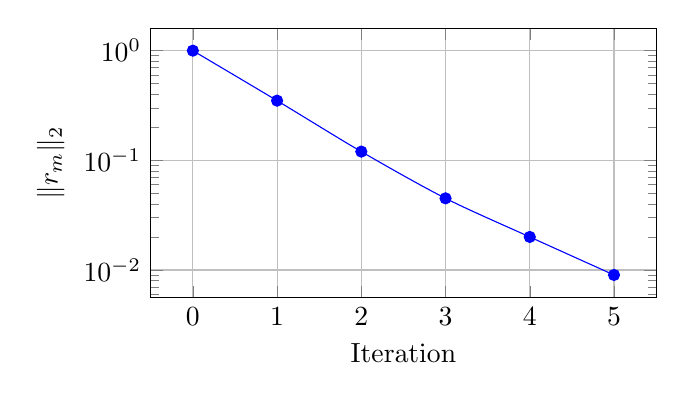
\begin{tikzpicture}
  \begin{semilogyaxis}[
    xlabel=Iteration,
    ylabel={$\|r_m\|_2$},
    grid=major,
    width=8cm,
    height=5cm
  ]
    % Sample decay curve (replace with actual data if desired)
    \addplot[smooth,mark=*,blue] coordinates {
      (0,1) (1,0.35) (2,0.12) (3,0.045) (4,0.02) (5,0.009)
    };
  \end{semilogyaxis}
\end{tikzpicture}
\end{document}

    \caption{Residual norm vs iteration for a typical GMRES run (see the runnable demo in \texttt{examples/gmres\_demo.py}).}
    \label{fig:gmres-residual}
\end{figure}
\begin{example}{GMRES example}{gmres-example}
Consider the system
\[
    A = \begin{bmatrix}4 & 1 & 2\\0 & 3 & -1\\1 & -1 & 2\end{bmatrix},\quad
    \mathbf{b} = \begin{bmatrix}1\\2\\0\end{bmatrix},\quad
    \mathbf{x}_0 = \begin{bmatrix}0\\0\\0\end{bmatrix}.
\]
The initial residual is $\mathbf{r}_0 = \mathbf{b} - A\mathbf{x}_0 = \mathbf{b}$ with norm $\beta = \|\mathbf{r}_0\|_2 = \sqrt{5}$.
The first Arnoldi vector is $\mathbf{v}_1 = \mathbf{r}_0 / \beta$. We perform the Arnoldi process to build the Krylov basis and Hessenberg matrix, applying Givens rotations to maintain the QR factorization. After $m$ steps, we solve the least-squares problem to find $\mathbf{y}_m$ and update the solution $\mathbf{x}_m = \mathbf{x}_0 + V_m \mathbf{y}_m$.
\end{example}

\section{Convergence of GMRES}
We give a standard polynomial-based bound. Let $\mathbf{x}_\star$ be the exact solution of $A\mathbf{x}=\mathbf{b}$ and let $\mathbf{x}_m$ be the iterate after $m$ steps of a Krylov method. Then there exists a polynomial $p_m\in\mathbb{P}_m$ with $p_m(0)=1$ such that
\[
    \mathbf{r}_m = \mathbf{b}-A\mathbf{x}_m = p_m(A)\mathbf{r}_0.
\]
If $A$ is diagonalizable, $A=X\Lambda X^{-1}$, then
\[
    \|\mathbf{r}_m\|_2 \le \|X\|_2\|X^{-1}\|_2 \max_{1\le i\le n} |p_m(\lambda_i)|\,\|\mathbf{r}_0\|_2
    = \kappa_2(X)\max_{\lambda\in\sigma(A)}|p_m(\lambda)|\,\|\mathbf{r}_0\|_2,
\]
where $\kappa_2(X)=\|X\|_2\|X^{-1}\|_2$.

Thus to bound GMRES one seeks
\[
    \min_{\substack{p\in\mathbb{P}_m\\ p(0)=1}}\max_{\lambda\in\mathrm{E}} |p(\lambda)|,
\]
where $\mathrm{E}$ is a compact region (often an ellipse) that contains the spectrum of $A$.

\subsubsection{Chebyshev polynomials (complex extension)}
For $z\in\mathbb{C}$ with $|z|>1$ one may use the analytic continuation of Chebyshev polynomials. With $\rho=\operatorname{arccosh}(z)$ and $w=e^\rho$,
\[
    C_m(z)=\cosh(m\rho)=\tfrac{1}{2}(w^m+w^{-m}),\quad z=\tfrac12(w+w^{-1}),
\]
and the three-term recurrence $C_{m+1}(z)=2zC_m(z)-C_{m-1}(z)$ holds.

\begin{lemma}{Zarantello}{zarantello}
    Let $\gamma\in\mathbb{C}$ with $|\gamma|>\rho$. Then
    \[
        \min_{\substack{p\in\mathbb{P}_m\\ p(\gamma)=1}}\max_{w\in D_\rho}|p(w)|=\left(\frac{\rho}{|\gamma|}\right)^m,
    \]
    and the minimizer is $p(z)=\big(\tfrac{z}{\gamma}\big)^m$ (maximum attained at $|z|=\rho$).
\end{lemma}

\subsubsection{Joukowsky map and ellipse bounds}
The Joukowsky map
\[
    J(w)=\tfrac12(w+w^{-1}),\quad w\in\mathbb{C}\setminus\{0\},
\]
maps the circle $D_\rho=\{w:|w|=\rho\}$ to an ellipse
\[
    J(D_\rho)=\mathrm{E}\big(0,1,\tfrac12(\rho+\rho^{-1})\big).
\]

\begin{theorem}{Elman}{elman}
    Let $J(D_\rho)=\mathrm{E}_\rho$ and choose $\gamma\not\in\mathrm{E}_\rho$. Let $w_\gamma$ be the preimage of $\gamma$ under $J$ with maximal modulus. Then
    \[
        \frac{\rho^m}{|w_\gamma|^m}
        \le
        \min_{\substack{p\in\mathbb{P}_m\\ p(\gamma)=1}}\max_{z\in\mathrm{E}_\rho}|p(z)|
        \le
        \frac{\rho^m+\rho^{-m}}{|w_\gamma^m+w_\gamma^{-m}|}.
    \]
    The near-optimal polynomial is
    \[
        p^\star(w)=\frac{w^m+w^{-m}}{w_\gamma^m+w_\gamma^{-m}},\qquad w\in\mathbb{C}.
    \]
\end{theorem}

For a general ellipse $\mathrm{E}(c,d,a)$ containing the spectrum, one can scale and shift the Chebyshev polynomial:
\[
    \widehat{C}_m(z)=\frac{C_m\big(\tfrac{z-c}{d}\big)}{C_m\big(-\tfrac{c}{d}\big)},\qquad \widehat{C}_m(0)=1,
\]
and obtain
\[
    \max_{z\in\mathrm{E}(c,d,a)}|\widehat{C}_m(z)|=\frac{C_m(\tfrac{a}{d})}{\big|C_m(-\tfrac{c}{d})\big|}.
\]
Therefore a practical bound for GMRES is
\[
    \|\mathbf{r}_m\|_2 \le \kappa_2(X)\,\varepsilon^m\,\|\mathbf{r}_0\|_2,
    \qquad
    \varepsilon^m=\frac{C_m(\tfrac{a}{d})}{\big|C_m(-\tfrac{c}{d})\big|}
    \approx \left(\frac{a+\sqrt{a^2-d^2}}{c+\sqrt{c^2-d^2}}\right)^m
\]
for large $m$.

Note: the ellipse enclosing the eigenvalues must not include $0$ (because $p(0)=1$ is required). If the ellipse is separated from the origin (e.g. $a<c$ in a standard parametrization) one obtains guaranteed geometric decay of the bound above.
